\chapter{Source Structure}

\section{Packages}

  \begin{figure}[h]
  \centering
  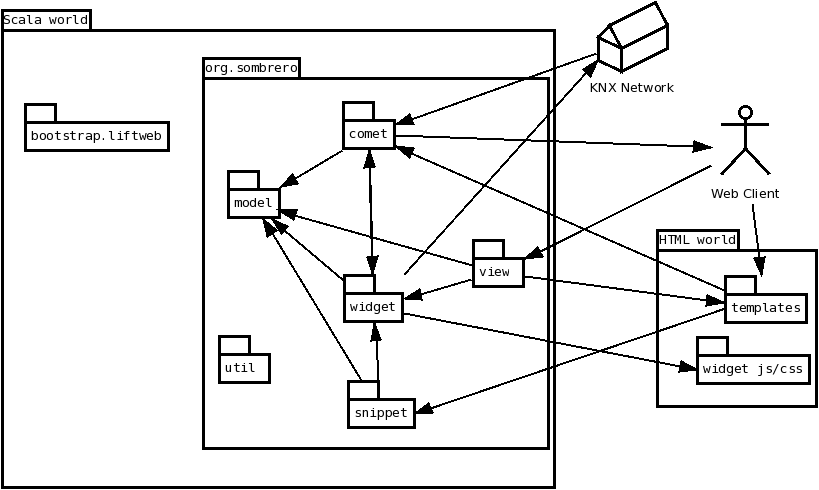
\includegraphics[width=0.80\linewidth]{packages.png}
  %% Graphic for TeX using PGF
% Title: /home/alex/Documents/Schule/Diplomarbeit/diplatex/dia/packages.dia
% Creator: Dia v0.97
% CreationDate: Mon May 17 13:12:52 2010
% For: alex
% \usepackage{tikz}
% The following commands are not supported in PSTricks at present
% We define them conditionally, so when they are implemented,
% this pgf file will use them.
\ifx\du\undefined
  \newlength{\du}
\fi
\setlength{\du}{15\unitlength}
\begin{tikzpicture}
\pgftransformxscale{1.000000}
\pgftransformyscale{-1.000000}
\definecolor{dialinecolor}{rgb}{0.000000, 0.000000, 0.000000}
\pgfsetstrokecolor{dialinecolor}
\definecolor{dialinecolor}{rgb}{1.000000, 1.000000, 1.000000}
\pgfsetfillcolor{dialinecolor}
\pgfsetlinewidth{0.150000\du}
\pgfsetdash{}{0pt}
\definecolor{dialinecolor}{rgb}{1.000000, 1.000000, 1.000000}
\pgfsetfillcolor{dialinecolor}
\fill (38.700000\du,12.850000\du)--(38.700000\du,20.650000\du)--(46.675000\du,20.650000\du)--(46.675000\du,12.850000\du)--cycle;
\definecolor{dialinecolor}{rgb}{0.000000, 0.000000, 0.000000}
\pgfsetstrokecolor{dialinecolor}
\draw (38.700000\du,12.850000\du)--(38.700000\du,20.650000\du)--(46.675000\du,20.650000\du)--(46.675000\du,12.850000\du)--cycle;
\definecolor{dialinecolor}{rgb}{1.000000, 1.000000, 1.000000}
\pgfsetfillcolor{dialinecolor}
\fill (38.700000\du,11.850000\du)--(38.700000\du,12.850000\du)--(42.750000\du,12.850000\du)--(42.750000\du,11.850000\du)--cycle;
\definecolor{dialinecolor}{rgb}{0.000000, 0.000000, 0.000000}
\pgfsetstrokecolor{dialinecolor}
\draw (38.700000\du,11.850000\du)--(38.700000\du,12.850000\du)--(42.750000\du,12.850000\du)--(42.750000\du,11.850000\du)--cycle;
% setfont left to latex
\definecolor{dialinecolor}{rgb}{0.000000, 0.000000, 0.000000}
\pgfsetstrokecolor{dialinecolor}
\node[anchor=west] at (38.800000\du,12.550000\du){HTML world};
\pgfsetlinewidth{0.150000\du}
\pgfsetdash{}{0pt}
\definecolor{dialinecolor}{rgb}{1.000000, 1.000000, 1.000000}
\pgfsetfillcolor{dialinecolor}
\fill (5.925000\du,1.850000\du)--(5.925000\du,24.700000\du)--(33.575000\du,24.700000\du)--(33.575000\du,1.850000\du)--cycle;
\definecolor{dialinecolor}{rgb}{0.000000, 0.000000, 0.000000}
\pgfsetstrokecolor{dialinecolor}
\draw (5.925000\du,1.850000\du)--(5.925000\du,24.700000\du)--(33.575000\du,24.700000\du)--(33.575000\du,1.850000\du)--cycle;
\definecolor{dialinecolor}{rgb}{1.000000, 1.000000, 1.000000}
\pgfsetfillcolor{dialinecolor}
\fill (5.925000\du,0.850000\du)--(5.925000\du,1.850000\du)--(10.360000\du,1.850000\du)--(10.360000\du,0.850000\du)--cycle;
\definecolor{dialinecolor}{rgb}{0.000000, 0.000000, 0.000000}
\pgfsetstrokecolor{dialinecolor}
\draw (5.925000\du,0.850000\du)--(5.925000\du,1.850000\du)--(10.360000\du,1.850000\du)--(10.360000\du,0.850000\du)--cycle;
% setfont left to latex
\definecolor{dialinecolor}{rgb}{0.000000, 0.000000, 0.000000}
\pgfsetstrokecolor{dialinecolor}
\node[anchor=west] at (6.025000\du,1.550000\du){Scala world};
\pgfsetlinewidth{0.150000\du}
\pgfsetdash{}{0pt}
\definecolor{dialinecolor}{rgb}{1.000000, 1.000000, 1.000000}
\pgfsetfillcolor{dialinecolor}
\fill (15.975000\du,4.250000\du)--(15.975000\du,22.750000\du)--(33.225000\du,22.750000\du)--(33.225000\du,4.250000\du)--cycle;
\definecolor{dialinecolor}{rgb}{0.000000, 0.000000, 0.000000}
\pgfsetstrokecolor{dialinecolor}
\draw (15.975000\du,4.250000\du)--(15.975000\du,22.750000\du)--(33.225000\du,22.750000\du)--(33.225000\du,4.250000\du)--cycle;
\definecolor{dialinecolor}{rgb}{1.000000, 1.000000, 1.000000}
\pgfsetfillcolor{dialinecolor}
\fill (15.975000\du,3.250000\du)--(15.975000\du,4.250000\du)--(20.795000\du,4.250000\du)--(20.795000\du,3.250000\du)--cycle;
\definecolor{dialinecolor}{rgb}{0.000000, 0.000000, 0.000000}
\pgfsetstrokecolor{dialinecolor}
\draw (15.975000\du,3.250000\du)--(15.975000\du,4.250000\du)--(20.795000\du,4.250000\du)--(20.795000\du,3.250000\du)--cycle;
% setfont left to latex
\definecolor{dialinecolor}{rgb}{0.000000, 0.000000, 0.000000}
\pgfsetstrokecolor{dialinecolor}
\node[anchor=west] at (16.075000\du,3.950000\du){org.sombrero};
\pgfsetlinewidth{0.150000\du}
\pgfsetdash{}{0pt}
\definecolor{dialinecolor}{rgb}{1.000000, 1.000000, 1.000000}
\pgfsetfillcolor{dialinecolor}
\fill (7.100000\du,6.450000\du)--(7.100000\du,7.850000\du)--(14.245000\du,7.850000\du)--(14.245000\du,6.450000\du)--cycle;
\definecolor{dialinecolor}{rgb}{0.000000, 0.000000, 0.000000}
\pgfsetstrokecolor{dialinecolor}
\draw (7.100000\du,6.450000\du)--(7.100000\du,7.850000\du)--(14.245000\du,7.850000\du)--(14.245000\du,6.450000\du)--cycle;
\definecolor{dialinecolor}{rgb}{1.000000, 1.000000, 1.000000}
\pgfsetfillcolor{dialinecolor}
\fill (7.100000\du,5.550000\du)--(7.100000\du,6.450000\du)--(8.600000\du,6.450000\du)--(8.600000\du,5.550000\du)--cycle;
\definecolor{dialinecolor}{rgb}{0.000000, 0.000000, 0.000000}
\pgfsetstrokecolor{dialinecolor}
\draw (7.100000\du,5.550000\du)--(7.100000\du,6.450000\du)--(8.600000\du,6.450000\du)--(8.600000\du,5.550000\du)--cycle;
% setfont left to latex
\definecolor{dialinecolor}{rgb}{0.000000, 0.000000, 0.000000}
\pgfsetstrokecolor{dialinecolor}
\node[anchor=west] at (7.400000\du,7.345000\du){bootstrap.liftweb};
\pgfsetlinewidth{0.150000\du}
\pgfsetdash{}{0pt}
\definecolor{dialinecolor}{rgb}{1.000000, 1.000000, 1.000000}
\pgfsetfillcolor{dialinecolor}
\fill (17.250000\du,9.800000\du)--(17.250000\du,11.200000\du)--(19.775000\du,11.200000\du)--(19.775000\du,9.800000\du)--cycle;
\definecolor{dialinecolor}{rgb}{0.000000, 0.000000, 0.000000}
\pgfsetstrokecolor{dialinecolor}
\draw (17.250000\du,9.800000\du)--(17.250000\du,11.200000\du)--(19.775000\du,11.200000\du)--(19.775000\du,9.800000\du)--cycle;
\definecolor{dialinecolor}{rgb}{1.000000, 1.000000, 1.000000}
\pgfsetfillcolor{dialinecolor}
\fill (17.250000\du,8.900000\du)--(17.250000\du,9.800000\du)--(18.750000\du,9.800000\du)--(18.750000\du,8.900000\du)--cycle;
\definecolor{dialinecolor}{rgb}{0.000000, 0.000000, 0.000000}
\pgfsetstrokecolor{dialinecolor}
\draw (17.250000\du,8.900000\du)--(17.250000\du,9.800000\du)--(18.750000\du,9.800000\du)--(18.750000\du,8.900000\du)--cycle;
% setfont left to latex
\definecolor{dialinecolor}{rgb}{0.000000, 0.000000, 0.000000}
\pgfsetstrokecolor{dialinecolor}
\node[anchor=west] at (17.550000\du,10.695000\du){model};
\pgfsetlinewidth{0.150000\du}
\pgfsetdash{}{0pt}
\definecolor{dialinecolor}{rgb}{1.000000, 1.000000, 1.000000}
\pgfsetfillcolor{dialinecolor}
\fill (23.000000\du,6.350000\du)--(23.000000\du,7.750000\du)--(25.525000\du,7.750000\du)--(25.525000\du,6.350000\du)--cycle;
\definecolor{dialinecolor}{rgb}{0.000000, 0.000000, 0.000000}
\pgfsetstrokecolor{dialinecolor}
\draw (23.000000\du,6.350000\du)--(23.000000\du,7.750000\du)--(25.525000\du,7.750000\du)--(25.525000\du,6.350000\du)--cycle;
\definecolor{dialinecolor}{rgb}{1.000000, 1.000000, 1.000000}
\pgfsetfillcolor{dialinecolor}
\fill (23.000000\du,5.450000\du)--(23.000000\du,6.350000\du)--(24.500000\du,6.350000\du)--(24.500000\du,5.450000\du)--cycle;
\definecolor{dialinecolor}{rgb}{0.000000, 0.000000, 0.000000}
\pgfsetstrokecolor{dialinecolor}
\draw (23.000000\du,5.450000\du)--(23.000000\du,6.350000\du)--(24.500000\du,6.350000\du)--(24.500000\du,5.450000\du)--cycle;
% setfont left to latex
\definecolor{dialinecolor}{rgb}{0.000000, 0.000000, 0.000000}
\pgfsetstrokecolor{dialinecolor}
\node[anchor=west] at (23.300000\du,7.245000\du){comet};
\pgfsetlinewidth{0.150000\du}
\pgfsetdash{}{0pt}
\definecolor{dialinecolor}{rgb}{1.000000, 1.000000, 1.000000}
\pgfsetfillcolor{dialinecolor}
\fill (23.050000\du,15.000000\du)--(23.050000\du,16.400000\du)--(25.960000\du,16.400000\du)--(25.960000\du,15.000000\du)--cycle;
\definecolor{dialinecolor}{rgb}{0.000000, 0.000000, 0.000000}
\pgfsetstrokecolor{dialinecolor}
\draw (23.050000\du,15.000000\du)--(23.050000\du,16.400000\du)--(25.960000\du,16.400000\du)--(25.960000\du,15.000000\du)--cycle;
\definecolor{dialinecolor}{rgb}{1.000000, 1.000000, 1.000000}
\pgfsetfillcolor{dialinecolor}
\fill (23.050000\du,14.100000\du)--(23.050000\du,15.000000\du)--(24.550000\du,15.000000\du)--(24.550000\du,14.100000\du)--cycle;
\definecolor{dialinecolor}{rgb}{0.000000, 0.000000, 0.000000}
\pgfsetstrokecolor{dialinecolor}
\draw (23.050000\du,14.100000\du)--(23.050000\du,15.000000\du)--(24.550000\du,15.000000\du)--(24.550000\du,14.100000\du)--cycle;
% setfont left to latex
\definecolor{dialinecolor}{rgb}{0.000000, 0.000000, 0.000000}
\pgfsetstrokecolor{dialinecolor}
\node[anchor=west] at (23.350000\du,15.895000\du){widget};
\pgfsetlinewidth{0.150000\du}
\pgfsetdash{}{0pt}
\definecolor{dialinecolor}{rgb}{1.000000, 1.000000, 1.000000}
\pgfsetfillcolor{dialinecolor}
\fill (23.250000\du,20.300000\du)--(23.250000\du,21.700000\du)--(26.545000\du,21.700000\du)--(26.545000\du,20.300000\du)--cycle;
\definecolor{dialinecolor}{rgb}{0.000000, 0.000000, 0.000000}
\pgfsetstrokecolor{dialinecolor}
\draw (23.250000\du,20.300000\du)--(23.250000\du,21.700000\du)--(26.545000\du,21.700000\du)--(26.545000\du,20.300000\du)--cycle;
\definecolor{dialinecolor}{rgb}{1.000000, 1.000000, 1.000000}
\pgfsetfillcolor{dialinecolor}
\fill (23.250000\du,19.400000\du)--(23.250000\du,20.300000\du)--(24.750000\du,20.300000\du)--(24.750000\du,19.400000\du)--cycle;
\definecolor{dialinecolor}{rgb}{0.000000, 0.000000, 0.000000}
\pgfsetstrokecolor{dialinecolor}
\draw (23.250000\du,19.400000\du)--(23.250000\du,20.300000\du)--(24.750000\du,20.300000\du)--(24.750000\du,19.400000\du)--cycle;
% setfont left to latex
\definecolor{dialinecolor}{rgb}{0.000000, 0.000000, 0.000000}
\pgfsetstrokecolor{dialinecolor}
\node[anchor=west] at (23.550000\du,21.195000\du){snippet};
\pgfsetlinewidth{0.150000\du}
\pgfsetdash{}{0pt}
\definecolor{dialinecolor}{rgb}{1.000000, 1.000000, 1.000000}
\pgfsetfillcolor{dialinecolor}
\fill (16.800000\du,18.050000\du)--(16.800000\du,19.450000\du)--(19.300000\du,19.450000\du)--(19.300000\du,18.050000\du)--cycle;
\definecolor{dialinecolor}{rgb}{0.000000, 0.000000, 0.000000}
\pgfsetstrokecolor{dialinecolor}
\draw (16.800000\du,18.050000\du)--(16.800000\du,19.450000\du)--(19.300000\du,19.450000\du)--(19.300000\du,18.050000\du)--cycle;
\definecolor{dialinecolor}{rgb}{1.000000, 1.000000, 1.000000}
\pgfsetfillcolor{dialinecolor}
\fill (16.800000\du,17.150000\du)--(16.800000\du,18.050000\du)--(18.300000\du,18.050000\du)--(18.300000\du,17.150000\du)--cycle;
\definecolor{dialinecolor}{rgb}{0.000000, 0.000000, 0.000000}
\pgfsetstrokecolor{dialinecolor}
\draw (16.800000\du,17.150000\du)--(16.800000\du,18.050000\du)--(18.300000\du,18.050000\du)--(18.300000\du,17.150000\du)--cycle;
% setfont left to latex
\definecolor{dialinecolor}{rgb}{0.000000, 0.000000, 0.000000}
\pgfsetstrokecolor{dialinecolor}
\node[anchor=west] at (17.100000\du,18.945000\du){util};
\pgfsetlinewidth{0.150000\du}
\pgfsetdash{}{0pt}
\definecolor{dialinecolor}{rgb}{1.000000, 1.000000, 1.000000}
\pgfsetfillcolor{dialinecolor}
\fill (29.500000\du,13.250000\du)--(29.500000\du,14.650000\du)--(32.000000\du,14.650000\du)--(32.000000\du,13.250000\du)--cycle;
\definecolor{dialinecolor}{rgb}{0.000000, 0.000000, 0.000000}
\pgfsetstrokecolor{dialinecolor}
\draw (29.500000\du,13.250000\du)--(29.500000\du,14.650000\du)--(32.000000\du,14.650000\du)--(32.000000\du,13.250000\du)--cycle;
\definecolor{dialinecolor}{rgb}{1.000000, 1.000000, 1.000000}
\pgfsetfillcolor{dialinecolor}
\fill (29.500000\du,12.350000\du)--(29.500000\du,13.250000\du)--(31.000000\du,13.250000\du)--(31.000000\du,12.350000\du)--cycle;
\definecolor{dialinecolor}{rgb}{0.000000, 0.000000, 0.000000}
\pgfsetstrokecolor{dialinecolor}
\draw (29.500000\du,12.350000\du)--(29.500000\du,13.250000\du)--(31.000000\du,13.250000\du)--(31.000000\du,12.350000\du)--cycle;
% setfont left to latex
\definecolor{dialinecolor}{rgb}{0.000000, 0.000000, 0.000000}
\pgfsetstrokecolor{dialinecolor}
\node[anchor=west] at (29.800000\du,14.145000\du){view};
\pgfsetlinewidth{0.150000\du}
\pgfsetdash{}{0pt}
\definecolor{dialinecolor}{rgb}{1.000000, 1.000000, 1.000000}
\pgfsetfillcolor{dialinecolor}
\fill (42.100000\du,15.050000\du)--(42.100000\du,16.450000\du)--(46.165000\du,16.450000\du)--(46.165000\du,15.050000\du)--cycle;
\definecolor{dialinecolor}{rgb}{0.000000, 0.000000, 0.000000}
\pgfsetstrokecolor{dialinecolor}
\draw (42.100000\du,15.050000\du)--(42.100000\du,16.450000\du)--(46.165000\du,16.450000\du)--(46.165000\du,15.050000\du)--cycle;
\definecolor{dialinecolor}{rgb}{1.000000, 1.000000, 1.000000}
\pgfsetfillcolor{dialinecolor}
\fill (42.100000\du,14.150000\du)--(42.100000\du,15.050000\du)--(43.600000\du,15.050000\du)--(43.600000\du,14.150000\du)--cycle;
\definecolor{dialinecolor}{rgb}{0.000000, 0.000000, 0.000000}
\pgfsetstrokecolor{dialinecolor}
\draw (42.100000\du,14.150000\du)--(42.100000\du,15.050000\du)--(43.600000\du,15.050000\du)--(43.600000\du,14.150000\du)--cycle;
% setfont left to latex
\definecolor{dialinecolor}{rgb}{0.000000, 0.000000, 0.000000}
\pgfsetstrokecolor{dialinecolor}
\node[anchor=west] at (42.400000\du,15.945000\du){templates};
\pgfsetlinewidth{0.150000\du}
\pgfsetdash{}{0pt}
\definecolor{dialinecolor}{rgb}{1.000000, 1.000000, 1.000000}
\pgfsetfillcolor{dialinecolor}
\fill (40.700000\du,18.100000\du)--(40.700000\du,19.500000\du)--(46.305000\du,19.500000\du)--(46.305000\du,18.100000\du)--cycle;
\definecolor{dialinecolor}{rgb}{0.000000, 0.000000, 0.000000}
\pgfsetstrokecolor{dialinecolor}
\draw (40.700000\du,18.100000\du)--(40.700000\du,19.500000\du)--(46.305000\du,19.500000\du)--(46.305000\du,18.100000\du)--cycle;
\definecolor{dialinecolor}{rgb}{1.000000, 1.000000, 1.000000}
\pgfsetfillcolor{dialinecolor}
\fill (40.700000\du,17.200000\du)--(40.700000\du,18.100000\du)--(42.200000\du,18.100000\du)--(42.200000\du,17.200000\du)--cycle;
\definecolor{dialinecolor}{rgb}{0.000000, 0.000000, 0.000000}
\pgfsetstrokecolor{dialinecolor}
\draw (40.700000\du,17.200000\du)--(40.700000\du,18.100000\du)--(42.200000\du,18.100000\du)--(42.200000\du,17.200000\du)--cycle;
% setfont left to latex
\definecolor{dialinecolor}{rgb}{0.000000, 0.000000, 0.000000}
\pgfsetstrokecolor{dialinecolor}
\node[anchor=west] at (41.000000\du,18.995000\du){widget js/css};
\pgfsetlinewidth{0.100000\du}
\pgfsetbuttcap
\pgfsetdash{}{0pt}
{
\definecolor{dialinecolor}{rgb}{0.000000, 0.000000, 0.000000}
\pgfsetfillcolor{dialinecolor}
% was here!!!
\pgfsetarrowsstart{latex}
\definecolor{dialinecolor}{rgb}{0.000000, 0.000000, 0.000000}
\pgfsetstrokecolor{dialinecolor}
\draw (26.545000\du,21.000000\du)--(42.100000\du,15.750000\du);
}
% setfont left to latex
\pgfsetlinewidth{0.100000\du}
\pgfsetbuttcap
\pgfsetdash{}{0pt}
{
\definecolor{dialinecolor}{rgb}{0.000000, 0.000000, 0.000000}
\pgfsetfillcolor{dialinecolor}
% was here!!!
\pgfsetarrowsstart{latex}
\definecolor{dialinecolor}{rgb}{0.000000, 0.000000, 0.000000}
\pgfsetstrokecolor{dialinecolor}
\draw (24.562351\du,16.474426\du)--(24.773454\du,19.324988\du);
}
% setfont left to latex
\pgfsetlinewidth{0.100000\du}
\pgfsetbuttcap
\pgfsetdash{}{0pt}
{
\definecolor{dialinecolor}{rgb}{0.000000, 0.000000, 0.000000}
\pgfsetfillcolor{dialinecolor}
% was here!!!
\pgfsetarrowsstart{latex}
\definecolor{dialinecolor}{rgb}{0.000000, 0.000000, 0.000000}
\pgfsetstrokecolor{dialinecolor}
\draw (40.700000\du,18.800000\du)--(26.033166\du,15.992517\du);
}
% setfont left to latex
\pgfsetlinewidth{0.100000\du}
\pgfsetbuttcap
\pgfsetdash{}{0pt}
{
\definecolor{dialinecolor}{rgb}{0.000000, 0.000000, 0.000000}
\pgfsetfillcolor{dialinecolor}
% was here!!!
\pgfsetarrowsstart{latex}
\definecolor{dialinecolor}{rgb}{0.000000, 0.000000, 0.000000}
\pgfsetstrokecolor{dialinecolor}
\draw (26.032708\du,15.271899\du)--(29.424691\du,14.321384\du);
}
% setfont left to latex
\pgfsetlinewidth{0.150000\du}
\pgfsetdash{}{0pt}
\definecolor{dialinecolor}{rgb}{1.000000, 1.000000, 1.000000}
\pgfsetfillcolor{dialinecolor}
\pgfpathellipse{\pgfpoint{43.100000\du}{5.950000\du}}{\pgfpoint{0.300000\du}{0\du}}{\pgfpoint{0\du}{0.300000\du}}
\pgfusepath{fill}
\definecolor{dialinecolor}{rgb}{0.000000, 0.000000, 0.000000}
\pgfsetstrokecolor{dialinecolor}
\pgfpathellipse{\pgfpoint{43.100000\du}{5.950000\du}}{\pgfpoint{0.300000\du}{0\du}}{\pgfpoint{0\du}{0.300000\du}}
\pgfusepath{stroke}
\definecolor{dialinecolor}{rgb}{0.000000, 0.000000, 0.000000}
\pgfsetstrokecolor{dialinecolor}
\draw (41.900000\du,6.550000\du)--(44.300000\du,6.550000\du);
\definecolor{dialinecolor}{rgb}{0.000000, 0.000000, 0.000000}
\pgfsetstrokecolor{dialinecolor}
\draw (43.100000\du,6.250000\du)--(43.100000\du,7.750000\du);
\definecolor{dialinecolor}{rgb}{0.000000, 0.000000, 0.000000}
\pgfsetstrokecolor{dialinecolor}
\draw (43.100000\du,7.750000\du)--(41.900000\du,9.050000\du);
\definecolor{dialinecolor}{rgb}{0.000000, 0.000000, 0.000000}
\pgfsetstrokecolor{dialinecolor}
\draw (43.100000\du,7.750000\du)--(44.300000\du,9.050000\du);
% setfont left to latex
\definecolor{dialinecolor}{rgb}{0.000000, 0.000000, 0.000000}
\pgfsetstrokecolor{dialinecolor}
\node at (43.100000\du,10.245000\du){Web Client};
\pgfsetlinewidth{0.100000\du}
\pgfsetbuttcap
\pgfsetdash{}{0pt}
{
\definecolor{dialinecolor}{rgb}{0.000000, 0.000000, 0.000000}
\pgfsetfillcolor{dialinecolor}
% was here!!!
\pgfsetarrowsstart{latex}
\definecolor{dialinecolor}{rgb}{0.000000, 0.000000, 0.000000}
\pgfsetstrokecolor{dialinecolor}
\draw (43.916472\du,14.076172\du)--(43.458073\du,10.524414\du);
}
% setfont left to latex
\pgfsetlinewidth{0.100000\du}
\pgfsetbuttcap
\pgfsetdash{}{0pt}
{
\definecolor{dialinecolor}{rgb}{0.000000, 0.000000, 0.000000}
\pgfsetfillcolor{dialinecolor}
% was here!!!
\pgfsetarrowsstart{latex}
\definecolor{dialinecolor}{rgb}{0.000000, 0.000000, 0.000000}
\pgfsetstrokecolor{dialinecolor}
\draw (41.377675\du,7.685999\du)--(25.598509\du,7.099646\du);
}
% setfont left to latex
\pgfsetlinewidth{0.100000\du}
\pgfsetbuttcap
\pgfsetdash{}{0pt}
{
\definecolor{dialinecolor}{rgb}{0.000000, 0.000000, 0.000000}
\pgfsetfillcolor{dialinecolor}
% was here!!!
\pgfsetarrowsstart{latex}
\definecolor{dialinecolor}{rgb}{0.000000, 0.000000, 0.000000}
\pgfsetstrokecolor{dialinecolor}
\draw (32.074399\du,13.285120\du)--(41.381372\du,8.612793\du);
}
% setfont left to latex
\pgfsetlinewidth{0.150000\du}
\pgfsetdash{}{0pt}
\pgfsetdash{}{0pt}
\pgfsetbuttcap
\pgfsetmiterjoin
\pgfsetlinewidth{0.150000\du}
\pgfsetbuttcap
\pgfsetmiterjoin
\pgfsetdash{}{0pt}
\definecolor{dialinecolor}{rgb}{1.000000, 1.000000, 1.000000}
\pgfsetfillcolor{dialinecolor}
\fill (36.311783\du,1.604167\du)--(36.888867\du,2.758333\du)--(35.734700\du,2.181250\du)--cycle;
\definecolor{dialinecolor}{rgb}{0.000000, 0.000000, 0.000000}
\pgfsetstrokecolor{dialinecolor}
\draw (36.311783\du,1.604167\du)--(36.888867\du,2.758333\du)--(35.734700\du,2.181250\du)--cycle;
\pgfsetlinewidth{0.015000\du}
\pgfsetbuttcap
\pgfsetmiterjoin
\pgfsetdash{}{0pt}
\definecolor{dialinecolor}{rgb}{0.000000, 0.000000, 0.000000}
\pgfsetstrokecolor{dialinecolor}
\draw (36.311783\du,1.604167\du)--(36.888867\du,2.758333\du)--(35.734700\du,2.181250\du)--cycle;
\pgfsetlinewidth{0.150000\du}
\pgfsetbuttcap
\pgfsetmiterjoin
\pgfsetdash{}{0pt}
\definecolor{dialinecolor}{rgb}{1.000000, 1.000000, 1.000000}
\pgfsetfillcolor{dialinecolor}
\fill (38.620117\du,0.450000\du)--(39.197200\du,1.604167\du)--(36.888867\du,2.758333\du)--(36.311783\du,1.604167\du)--cycle;
\definecolor{dialinecolor}{rgb}{0.000000, 0.000000, 0.000000}
\pgfsetstrokecolor{dialinecolor}
\draw (38.620117\du,0.450000\du)--(39.197200\du,1.604167\du)--(36.888867\du,2.758333\du)--(36.311783\du,1.604167\du)--cycle;
\pgfsetlinewidth{0.015000\du}
\pgfsetbuttcap
\pgfsetmiterjoin
\pgfsetdash{}{0pt}
\definecolor{dialinecolor}{rgb}{0.000000, 0.000000, 0.000000}
\pgfsetstrokecolor{dialinecolor}
\draw (38.620117\du,0.450000\du)--(39.197200\du,1.604167\du)--(36.888867\du,2.758333\du)--(36.311783\du,1.604167\du)--cycle;
\pgfsetlinewidth{0.150000\du}
\pgfsetbuttcap
\pgfsetmiterjoin
\pgfsetdash{}{0pt}
\definecolor{dialinecolor}{rgb}{1.000000, 1.000000, 1.000000}
\pgfsetfillcolor{dialinecolor}
\fill (35.734700\du,2.181250\du)--(36.888867\du,2.758333\du)--(36.888867\du,3.912500\du)--(35.734700\du,3.335417\du)--cycle;
\definecolor{dialinecolor}{rgb}{0.000000, 0.000000, 0.000000}
\pgfsetstrokecolor{dialinecolor}
\draw (35.734700\du,2.181250\du)--(36.888867\du,2.758333\du)--(36.888867\du,3.912500\du)--(35.734700\du,3.335417\du)--cycle;
\pgfsetlinewidth{0.015000\du}
\pgfsetbuttcap
\pgfsetmiterjoin
\pgfsetdash{}{0pt}
\definecolor{dialinecolor}{rgb}{0.000000, 0.000000, 0.000000}
\pgfsetstrokecolor{dialinecolor}
\draw (35.734700\du,2.181250\du)--(36.888867\du,2.758333\du)--(36.888867\du,3.912500\du)--(35.734700\du,3.335417\du)--cycle;
\pgfsetlinewidth{0.150000\du}
\pgfsetbuttcap
\pgfsetmiterjoin
\pgfsetdash{}{0pt}
\definecolor{dialinecolor}{rgb}{1.000000, 1.000000, 1.000000}
\pgfsetfillcolor{dialinecolor}
\fill (36.888867\du,2.758333\du)--(39.197200\du,1.604167\du)--(39.197200\du,2.758333\du)--(36.888867\du,3.912500\du)--cycle;
\definecolor{dialinecolor}{rgb}{0.000000, 0.000000, 0.000000}
\pgfsetstrokecolor{dialinecolor}
\draw (36.888867\du,2.758333\du)--(39.197200\du,1.604167\du)--(39.197200\du,2.758333\du)--(36.888867\du,3.912500\du)--cycle;
\pgfsetlinewidth{0.015000\du}
\pgfsetbuttcap
\pgfsetmiterjoin
\pgfsetdash{}{0pt}
\definecolor{dialinecolor}{rgb}{0.000000, 0.000000, 0.000000}
\pgfsetstrokecolor{dialinecolor}
\draw (36.888867\du,2.758333\du)--(39.197200\du,1.604167\du)--(39.197200\du,2.758333\du)--(36.888867\du,3.912500\du)--cycle;
% setfont left to latex
\definecolor{dialinecolor}{rgb}{0.000000, 0.000000, 0.000000}
\pgfsetstrokecolor{dialinecolor}
\node[anchor=west] at (35.349200\du,4.950000\du){KNX Network};
\pgfsetlinewidth{0.100000\du}
\pgfsetbuttcap
\pgfsetdash{}{0pt}
{
\definecolor{dialinecolor}{rgb}{0.000000, 0.000000, 0.000000}
\pgfsetfillcolor{dialinecolor}
% was here!!!
\pgfsetarrowsstart{latex}
\definecolor{dialinecolor}{rgb}{0.000000, 0.000000, 0.000000}
\pgfsetstrokecolor{dialinecolor}
\draw (25.599903\du,6.575106\du)--(35.661153\du,3.002486\du);
}
% setfont left to latex
\pgfsetlinewidth{0.100000\du}
\pgfsetbuttcap
\pgfsetdash{}{0pt}
{
\definecolor{dialinecolor}{rgb}{0.000000, 0.000000, 0.000000}
\pgfsetfillcolor{dialinecolor}
% was here!!!
\pgfsetarrowsstart{latex}
\definecolor{dialinecolor}{rgb}{0.000000, 0.000000, 0.000000}
\pgfsetstrokecolor{dialinecolor}
\draw (25.599577\du,7.635434\du)--(42.025921\du,14.827643\du);
}
% setfont left to latex
\pgfsetlinewidth{0.100000\du}
\pgfsetbuttcap
\pgfsetdash{}{0pt}
{
\definecolor{dialinecolor}{rgb}{0.000000, 0.000000, 0.000000}
\pgfsetfillcolor{dialinecolor}
% was here!!!
\pgfsetarrowsstart{latex}
\definecolor{dialinecolor}{rgb}{0.000000, 0.000000, 0.000000}
\pgfsetstrokecolor{dialinecolor}
\draw (35.734700\du,3.335420\du)--(26.025232\du,14.026133\du);
}
% setfont left to latex
\pgfsetlinewidth{0.100000\du}
\pgfsetbuttcap
\pgfsetdash{}{0pt}
{
\definecolor{dialinecolor}{rgb}{0.000000, 0.000000, 0.000000}
\pgfsetfillcolor{dialinecolor}
% was here!!!
\pgfsetarrowsstart{latex}
\definecolor{dialinecolor}{rgb}{0.000000, 0.000000, 0.000000}
\pgfsetstrokecolor{dialinecolor}
\draw (24.284198\du,7.823981\du)--(24.458036\du,14.024802\du);
}
% setfont left to latex
\pgfsetlinewidth{0.100000\du}
\pgfsetbuttcap
\pgfsetdash{}{0pt}
{
\definecolor{dialinecolor}{rgb}{0.000000, 0.000000, 0.000000}
\pgfsetfillcolor{dialinecolor}
% was here!!!
\pgfsetarrowsstart{latex}
\definecolor{dialinecolor}{rgb}{0.000000, 0.000000, 0.000000}
\pgfsetstrokecolor{dialinecolor}
\draw (24.458036\du,14.024802\du)--(24.284198\du,7.823981\du);
}
% setfont left to latex
\pgfsetlinewidth{0.100000\du}
\pgfsetbuttcap
\pgfsetdash{}{0pt}
{
\definecolor{dialinecolor}{rgb}{0.000000, 0.000000, 0.000000}
\pgfsetfillcolor{dialinecolor}
% was here!!!
\pgfsetarrowsstart{latex}
\definecolor{dialinecolor}{rgb}{0.000000, 0.000000, 0.000000}
\pgfsetstrokecolor{dialinecolor}
\draw (18.983659\du,11.274811\du)--(23.879189\du,19.325409\du);
}
% setfont left to latex
\pgfsetlinewidth{0.100000\du}
\pgfsetbuttcap
\pgfsetdash{}{0pt}
{
\definecolor{dialinecolor}{rgb}{0.000000, 0.000000, 0.000000}
\pgfsetfillcolor{dialinecolor}
% was here!!!
\pgfsetarrowsstart{latex}
\definecolor{dialinecolor}{rgb}{0.000000, 0.000000, 0.000000}
\pgfsetstrokecolor{dialinecolor}
\draw (42.024740\du,15.466498\du)--(32.075263\du,14.128253\du);
}
% setfont left to latex
\pgfsetlinewidth{0.100000\du}
\pgfsetbuttcap
\pgfsetdash{}{0pt}
{
\definecolor{dialinecolor}{rgb}{0.000000, 0.000000, 0.000000}
\pgfsetfillcolor{dialinecolor}
% was here!!!
\pgfsetarrowsstart{latex}
\definecolor{dialinecolor}{rgb}{0.000000, 0.000000, 0.000000}
\pgfsetstrokecolor{dialinecolor}
\draw (19.405669\du,11.275049\du)--(22.976152\du,14.373340\du);
}
% setfont left to latex
\pgfsetlinewidth{0.100000\du}
\pgfsetbuttcap
\pgfsetdash{}{0pt}
{
\definecolor{dialinecolor}{rgb}{0.000000, 0.000000, 0.000000}
\pgfsetfillcolor{dialinecolor}
% was here!!!
\pgfsetarrowsstart{latex}
\definecolor{dialinecolor}{rgb}{0.000000, 0.000000, 0.000000}
\pgfsetstrokecolor{dialinecolor}
\draw (19.755371\du,10.850391\du)--(29.425715\du,13.576657\du);
}
% setfont left to latex
\pgfsetlinewidth{0.100000\du}
\pgfsetbuttcap
\pgfsetdash{}{0pt}
{
\definecolor{dialinecolor}{rgb}{0.000000, 0.000000, 0.000000}
\pgfsetfillcolor{dialinecolor}
% was here!!!
\pgfsetarrowsstart{latex}
\definecolor{dialinecolor}{rgb}{0.000000, 0.000000, 0.000000}
\pgfsetstrokecolor{dialinecolor}
\draw (19.849628\du,9.697723\du)--(22.970294\du,7.825323\du);
}
% setfont left to latex
\end{tikzpicture}

  \caption{package structure}
  \label{fig:packages}
  \end{figure}

This picture probably needs explanation. The Scala world is located under \lstinline!src/main/scala/!. The templates of HTML world are in \lstinline!src/main/webapp/!, the widget resources are in \lstinline!src/main/resources/toserve/!.

The user accesses Sombrero through a web browser. His request either matches one of the externally accessible templates or gets caught by URL rewriting of one of the location classes in the \lstinline!view! package, which will in turn redirect to a template, but supply it with special snippets. The most notable example for URL rewriting would be the room view. The user's request gets rewritten by the \lstinline!RoomLoc! class in \lstinline!view!, which redirects to \lstinline!room.html!, which in turn uses the \lstinline!roomview! snippet in \lstinline!RoomLoc!. \lstinline!RoomLoc! can then proceed, using information saved from the user's original request, to get widget information from the database interface that is the \lstinline!model! package and use it to construct the widgets that make up the room, using \lstinline!widget!'s various UI classes.

Templates can use other snippets, which don't depend on the user's request, too, these are located in the \lstinline!snippet! package. The favorites bar would be an example of such a snippet. KNX widgets use the KNX network to query the device status upon creation and forward the user's actions to the actual devices. The database is used to save widget positions. The \lstinline!comet! package includes everything that pushes data back to the user. This includes data about status changes in the KNX network, which is translated into UI changes by the widgets. The util package includes utility functionality used by every package (drawing all the arrows would have seriously impacted the clarity of the image), most notably the \lstinline!JavaScriptHelper! and the \lstinline!WidgetList!. Finally, the \lstinline!bootstrap.liftweb! package includes a single class, \lstinline!Boot!, which holds the Lift configuration.


\section{Database Model}

Because we use Lift's Mapper ORM framewrok, all database tables are represented by classes and their companion objects. These classes reside in the \lstinline!model! package. Note that although every Mapper class needs a companion object, they have been omitted in the following diagram for better readability. Many-to-many-relations have been implemented as seperate entities.

  \begin{figure}[h]
  \centering
  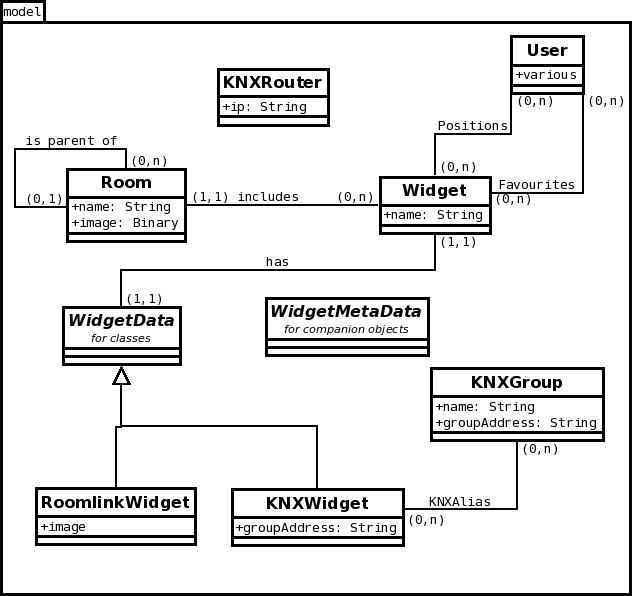
\includegraphics[width=0.80\linewidth]{model.png}
  %% Graphic for TeX using PGF
% Title: /home/alex/Documents/Schule/Diplomarbeit/diplatex/dia/model.dia
% Creator: Dia v0.97
% CreationDate: Mon May 17 13:13:05 2010
% For: alex
% \usepackage{tikz}
% The following commands are not supported in PSTricks at present
% We define them conditionally, so when they are implemented,
% this pgf file will use them.
\ifx\du\undefined
  \newlength{\du}
\fi
\setlength{\du}{15\unitlength}
\begin{tikzpicture}
\pgftransformxscale{1.000000}
\pgftransformyscale{-1.000000}
\definecolor{dialinecolor}{rgb}{0.000000, 0.000000, 0.000000}
\pgfsetstrokecolor{dialinecolor}
\definecolor{dialinecolor}{rgb}{1.000000, 1.000000, 1.000000}
\pgfsetfillcolor{dialinecolor}
\pgfsetlinewidth{0.150000\du}
\pgfsetdash{}{0pt}
\definecolor{dialinecolor}{rgb}{1.000000, 1.000000, 1.000000}
\pgfsetfillcolor{dialinecolor}
\fill (15.300000\du,1.300000\du)--(15.300000\du,29.900000\du)--(46.750000\du,29.900000\du)--(46.750000\du,1.300000\du)--cycle;
\definecolor{dialinecolor}{rgb}{0.000000, 0.000000, 0.000000}
\pgfsetstrokecolor{dialinecolor}
\draw (15.300000\du,1.300000\du)--(15.300000\du,29.900000\du)--(46.750000\du,29.900000\du)--(46.750000\du,1.300000\du)--cycle;
\definecolor{dialinecolor}{rgb}{1.000000, 1.000000, 1.000000}
\pgfsetfillcolor{dialinecolor}
\fill (15.300000\du,0.300000\du)--(15.300000\du,1.300000\du)--(17.425000\du,1.300000\du)--(17.425000\du,0.300000\du)--cycle;
\definecolor{dialinecolor}{rgb}{0.000000, 0.000000, 0.000000}
\pgfsetstrokecolor{dialinecolor}
\draw (15.300000\du,0.300000\du)--(15.300000\du,1.300000\du)--(17.425000\du,1.300000\du)--(17.425000\du,0.300000\du)--cycle;
% setfont left to latex
\definecolor{dialinecolor}{rgb}{0.000000, 0.000000, 0.000000}
\pgfsetstrokecolor{dialinecolor}
\node[anchor=west] at (15.400000\du,1.000000\du){model};
\pgfsetlinewidth{0.150000\du}
\pgfsetdash{}{0pt}
\definecolor{dialinecolor}{rgb}{1.000000, 1.000000, 1.000000}
\pgfsetfillcolor{dialinecolor}
\fill (18.600000\du,8.650000\du)--(18.600000\du,10.050000\du)--(24.490000\du,10.050000\du)--(24.490000\du,8.650000\du)--cycle;
\definecolor{dialinecolor}{rgb}{0.000000, 0.000000, 0.000000}
\pgfsetstrokecolor{dialinecolor}
\draw (18.600000\du,8.650000\du)--(18.600000\du,10.050000\du)--(24.490000\du,10.050000\du)--(24.490000\du,8.650000\du)--cycle;
% setfont left to latex
\definecolor{dialinecolor}{rgb}{0.000000, 0.000000, 0.000000}
\pgfsetstrokecolor{dialinecolor}
\node at (21.545000\du,9.600000\du){Room};
\definecolor{dialinecolor}{rgb}{1.000000, 1.000000, 1.000000}
\pgfsetfillcolor{dialinecolor}
\fill (18.600000\du,10.050000\du)--(18.600000\du,11.850000\du)--(24.490000\du,11.850000\du)--(24.490000\du,10.050000\du)--cycle;
\definecolor{dialinecolor}{rgb}{0.000000, 0.000000, 0.000000}
\pgfsetstrokecolor{dialinecolor}
\draw (18.600000\du,10.050000\du)--(18.600000\du,11.850000\du)--(24.490000\du,11.850000\du)--(24.490000\du,10.050000\du)--cycle;
% setfont left to latex
\definecolor{dialinecolor}{rgb}{0.000000, 0.000000, 0.000000}
\pgfsetstrokecolor{dialinecolor}
\node[anchor=west] at (18.775000\du,10.750000\du){+name: String};
% setfont left to latex
\definecolor{dialinecolor}{rgb}{0.000000, 0.000000, 0.000000}
\pgfsetstrokecolor{dialinecolor}
\node[anchor=west] at (18.775000\du,11.550000\du){+image: Binary};
\definecolor{dialinecolor}{rgb}{1.000000, 1.000000, 1.000000}
\pgfsetfillcolor{dialinecolor}
\fill (18.600000\du,11.850000\du)--(18.600000\du,12.250000\du)--(24.490000\du,12.250000\du)--(24.490000\du,11.850000\du)--cycle;
\definecolor{dialinecolor}{rgb}{0.000000, 0.000000, 0.000000}
\pgfsetstrokecolor{dialinecolor}
\draw (18.600000\du,11.850000\du)--(18.600000\du,12.250000\du)--(24.490000\du,12.250000\du)--(24.490000\du,11.850000\du)--cycle;
\pgfsetlinewidth{0.150000\du}
\pgfsetdash{}{0pt}
\definecolor{dialinecolor}{rgb}{1.000000, 1.000000, 1.000000}
\pgfsetfillcolor{dialinecolor}
\fill (34.200000\du,9.050000\du)--(34.200000\du,10.450000\du)--(39.705000\du,10.450000\du)--(39.705000\du,9.050000\du)--cycle;
\definecolor{dialinecolor}{rgb}{0.000000, 0.000000, 0.000000}
\pgfsetstrokecolor{dialinecolor}
\draw (34.200000\du,9.050000\du)--(34.200000\du,10.450000\du)--(39.705000\du,10.450000\du)--(39.705000\du,9.050000\du)--cycle;
% setfont left to latex
\definecolor{dialinecolor}{rgb}{0.000000, 0.000000, 0.000000}
\pgfsetstrokecolor{dialinecolor}
\node at (36.952500\du,10.000000\du){Widget};
\definecolor{dialinecolor}{rgb}{1.000000, 1.000000, 1.000000}
\pgfsetfillcolor{dialinecolor}
\fill (34.200000\du,10.450000\du)--(34.200000\du,11.450000\du)--(39.705000\du,11.450000\du)--(39.705000\du,10.450000\du)--cycle;
\definecolor{dialinecolor}{rgb}{0.000000, 0.000000, 0.000000}
\pgfsetstrokecolor{dialinecolor}
\draw (34.200000\du,10.450000\du)--(34.200000\du,11.450000\du)--(39.705000\du,11.450000\du)--(39.705000\du,10.450000\du)--cycle;
% setfont left to latex
\definecolor{dialinecolor}{rgb}{0.000000, 0.000000, 0.000000}
\pgfsetstrokecolor{dialinecolor}
\node[anchor=west] at (34.375000\du,11.150000\du){+name: String};
\definecolor{dialinecolor}{rgb}{1.000000, 1.000000, 1.000000}
\pgfsetfillcolor{dialinecolor}
\fill (34.200000\du,11.450000\du)--(34.200000\du,11.850000\du)--(39.705000\du,11.850000\du)--(39.705000\du,11.450000\du)--cycle;
\definecolor{dialinecolor}{rgb}{0.000000, 0.000000, 0.000000}
\pgfsetstrokecolor{dialinecolor}
\draw (34.200000\du,11.450000\du)--(34.200000\du,11.850000\du)--(39.705000\du,11.850000\du)--(39.705000\du,11.450000\du)--cycle;
\pgfsetlinewidth{0.150000\du}
\pgfsetdash{}{0pt}
\definecolor{dialinecolor}{rgb}{1.000000, 1.000000, 1.000000}
\pgfsetfillcolor{dialinecolor}
\fill (18.350000\du,15.550000\du)--(18.350000\du,17.650000\du)--(24.205000\du,17.650000\du)--(24.205000\du,15.550000\du)--cycle;
\definecolor{dialinecolor}{rgb}{0.000000, 0.000000, 0.000000}
\pgfsetstrokecolor{dialinecolor}
\draw (18.350000\du,15.550000\du)--(18.350000\du,17.650000\du)--(24.205000\du,17.650000\du)--(24.205000\du,15.550000\du)--cycle;
% setfont left to latex
\definecolor{dialinecolor}{rgb}{0.000000, 0.000000, 0.000000}
\pgfsetstrokecolor{dialinecolor}
\node at (21.277500\du,16.500000\du){WidgetData};
% setfont left to latex
\definecolor{dialinecolor}{rgb}{0.000000, 0.000000, 0.000000}
\pgfsetstrokecolor{dialinecolor}
\node at (21.277500\du,17.275000\du){for classes};
\definecolor{dialinecolor}{rgb}{1.000000, 1.000000, 1.000000}
\pgfsetfillcolor{dialinecolor}
\fill (18.350000\du,17.650000\du)--(18.350000\du,18.050000\du)--(24.205000\du,18.050000\du)--(24.205000\du,17.650000\du)--cycle;
\definecolor{dialinecolor}{rgb}{0.000000, 0.000000, 0.000000}
\pgfsetstrokecolor{dialinecolor}
\draw (18.350000\du,17.650000\du)--(18.350000\du,18.050000\du)--(24.205000\du,18.050000\du)--(24.205000\du,17.650000\du)--cycle;
\definecolor{dialinecolor}{rgb}{1.000000, 1.000000, 1.000000}
\pgfsetfillcolor{dialinecolor}
\fill (18.350000\du,18.050000\du)--(18.350000\du,18.450000\du)--(24.205000\du,18.450000\du)--(24.205000\du,18.050000\du)--cycle;
\definecolor{dialinecolor}{rgb}{0.000000, 0.000000, 0.000000}
\pgfsetstrokecolor{dialinecolor}
\draw (18.350000\du,18.050000\du)--(18.350000\du,18.450000\du)--(24.205000\du,18.450000\du)--(24.205000\du,18.050000\du)--cycle;
\pgfsetlinewidth{0.150000\du}
\pgfsetdash{}{0pt}
\definecolor{dialinecolor}{rgb}{1.000000, 1.000000, 1.000000}
\pgfsetfillcolor{dialinecolor}
\fill (28.500000\du,15.100000\du)--(28.500000\du,17.200000\du)--(36.615000\du,17.200000\du)--(36.615000\du,15.100000\du)--cycle;
\definecolor{dialinecolor}{rgb}{0.000000, 0.000000, 0.000000}
\pgfsetstrokecolor{dialinecolor}
\draw (28.500000\du,15.100000\du)--(28.500000\du,17.200000\du)--(36.615000\du,17.200000\du)--(36.615000\du,15.100000\du)--cycle;
% setfont left to latex
\definecolor{dialinecolor}{rgb}{0.000000, 0.000000, 0.000000}
\pgfsetstrokecolor{dialinecolor}
\node at (32.557500\du,16.050000\du){WidgetMetaData};
% setfont left to latex
\definecolor{dialinecolor}{rgb}{0.000000, 0.000000, 0.000000}
\pgfsetstrokecolor{dialinecolor}
\node at (32.557500\du,16.825000\du){for companion objects};
\definecolor{dialinecolor}{rgb}{1.000000, 1.000000, 1.000000}
\pgfsetfillcolor{dialinecolor}
\fill (28.500000\du,17.200000\du)--(28.500000\du,17.600000\du)--(36.615000\du,17.600000\du)--(36.615000\du,17.200000\du)--cycle;
\definecolor{dialinecolor}{rgb}{0.000000, 0.000000, 0.000000}
\pgfsetstrokecolor{dialinecolor}
\draw (28.500000\du,17.200000\du)--(28.500000\du,17.600000\du)--(36.615000\du,17.600000\du)--(36.615000\du,17.200000\du)--cycle;
\definecolor{dialinecolor}{rgb}{1.000000, 1.000000, 1.000000}
\pgfsetfillcolor{dialinecolor}
\fill (28.500000\du,17.600000\du)--(28.500000\du,18.000000\du)--(36.615000\du,18.000000\du)--(36.615000\du,17.600000\du)--cycle;
\definecolor{dialinecolor}{rgb}{0.000000, 0.000000, 0.000000}
\pgfsetstrokecolor{dialinecolor}
\draw (28.500000\du,17.600000\du)--(28.500000\du,18.000000\du)--(36.615000\du,18.000000\du)--(36.615000\du,17.600000\du)--cycle;
\pgfsetlinewidth{0.100000\du}
\pgfsetdash{}{0pt}
\pgfsetmiterjoin
\pgfsetbuttcap
{
\definecolor{dialinecolor}{rgb}{0.000000, 0.000000, 0.000000}
\pgfsetfillcolor{dialinecolor}
% was here!!!
\definecolor{dialinecolor}{rgb}{0.000000, 0.000000, 0.000000}
\pgfsetstrokecolor{dialinecolor}
\draw (34.127087\du,10.450000\du)--(26.950000\du,10.450000\du)--(26.950000\du,10.450000\du)--(24.564859\du,10.450000\du);
}
% setfont left to latex
\definecolor{dialinecolor}{rgb}{0.000000, 0.000000, 0.000000}
\pgfsetstrokecolor{dialinecolor}
\node at (26.950000\du,10.250000\du){includes};
\definecolor{dialinecolor}{rgb}{0.000000, 0.000000, 0.000000}
\pgfsetstrokecolor{dialinecolor}
\node[anchor=east] at (33.927087\du,10.250000\du){(0,n)};
\definecolor{dialinecolor}{rgb}{0.000000, 0.000000, 0.000000}
\pgfsetstrokecolor{dialinecolor}
\node[anchor=west] at (24.764859\du,10.250000\du){(1,1)};
\pgfsetlinewidth{0.100000\du}
\pgfsetdash{}{0pt}
\pgfsetmiterjoin
\pgfsetbuttcap
{
\definecolor{dialinecolor}{rgb}{0.000000, 0.000000, 0.000000}
\pgfsetfillcolor{dialinecolor}
% was here!!!
\definecolor{dialinecolor}{rgb}{0.000000, 0.000000, 0.000000}
\pgfsetstrokecolor{dialinecolor}
\draw (21.277500\du,15.550000\du)--(21.277500\du,13.737680\du)--(36.952500\du,13.737680\du)--(36.952500\du,11.925360\du);
}
% setfont left to latex
\definecolor{dialinecolor}{rgb}{0.000000, 0.000000, 0.000000}
\pgfsetstrokecolor{dialinecolor}
\node at (29.115000\du,13.537680\du){has};
\definecolor{dialinecolor}{rgb}{0.000000, 0.000000, 0.000000}
\pgfsetstrokecolor{dialinecolor}
\node[anchor=west] at (21.477500\du,15.350000\du){(1,1)};
\definecolor{dialinecolor}{rgb}{0.000000, 0.000000, 0.000000}
\pgfsetstrokecolor{dialinecolor}
\node[anchor=west] at (37.152500\du,12.525360\du){(1,1)};
\pgfsetlinewidth{0.150000\du}
\pgfsetdash{}{0pt}
\definecolor{dialinecolor}{rgb}{1.000000, 1.000000, 1.000000}
\pgfsetfillcolor{dialinecolor}
\fill (26.800000\du,24.700000\du)--(26.800000\du,26.100000\du)--(35.385000\du,26.100000\du)--(35.385000\du,24.700000\du)--cycle;
\definecolor{dialinecolor}{rgb}{0.000000, 0.000000, 0.000000}
\pgfsetstrokecolor{dialinecolor}
\draw (26.800000\du,24.700000\du)--(26.800000\du,26.100000\du)--(35.385000\du,26.100000\du)--(35.385000\du,24.700000\du)--cycle;
% setfont left to latex
\definecolor{dialinecolor}{rgb}{0.000000, 0.000000, 0.000000}
\pgfsetstrokecolor{dialinecolor}
\node at (31.092500\du,25.650000\du){KNXWidget};
\definecolor{dialinecolor}{rgb}{1.000000, 1.000000, 1.000000}
\pgfsetfillcolor{dialinecolor}
\fill (26.800000\du,26.100000\du)--(26.800000\du,27.100000\du)--(35.385000\du,27.100000\du)--(35.385000\du,26.100000\du)--cycle;
\definecolor{dialinecolor}{rgb}{0.000000, 0.000000, 0.000000}
\pgfsetstrokecolor{dialinecolor}
\draw (26.800000\du,26.100000\du)--(26.800000\du,27.100000\du)--(35.385000\du,27.100000\du)--(35.385000\du,26.100000\du)--cycle;
% setfont left to latex
\definecolor{dialinecolor}{rgb}{0.000000, 0.000000, 0.000000}
\pgfsetstrokecolor{dialinecolor}
\node[anchor=west] at (26.975000\du,26.800000\du){+groupAddress: String};
\definecolor{dialinecolor}{rgb}{1.000000, 1.000000, 1.000000}
\pgfsetfillcolor{dialinecolor}
\fill (26.800000\du,27.100000\du)--(26.800000\du,27.500000\du)--(35.385000\du,27.500000\du)--(35.385000\du,27.100000\du)--cycle;
\definecolor{dialinecolor}{rgb}{0.000000, 0.000000, 0.000000}
\pgfsetstrokecolor{dialinecolor}
\draw (26.800000\du,27.100000\du)--(26.800000\du,27.500000\du)--(35.385000\du,27.500000\du)--(35.385000\du,27.100000\du)--cycle;
\pgfsetlinewidth{0.150000\du}
\pgfsetdash{}{0pt}
\definecolor{dialinecolor}{rgb}{1.000000, 1.000000, 1.000000}
\pgfsetfillcolor{dialinecolor}
\fill (17.050000\du,24.650000\du)--(17.050000\du,26.050000\du)--(24.977500\du,26.050000\du)--(24.977500\du,24.650000\du)--cycle;
\definecolor{dialinecolor}{rgb}{0.000000, 0.000000, 0.000000}
\pgfsetstrokecolor{dialinecolor}
\draw (17.050000\du,24.650000\du)--(17.050000\du,26.050000\du)--(24.977500\du,26.050000\du)--(24.977500\du,24.650000\du)--cycle;
% setfont left to latex
\definecolor{dialinecolor}{rgb}{0.000000, 0.000000, 0.000000}
\pgfsetstrokecolor{dialinecolor}
\node at (21.013750\du,25.600000\du){RoomlinkWidget};
\definecolor{dialinecolor}{rgb}{1.000000, 1.000000, 1.000000}
\pgfsetfillcolor{dialinecolor}
\fill (17.050000\du,26.050000\du)--(17.050000\du,27.050000\du)--(24.977500\du,27.050000\du)--(24.977500\du,26.050000\du)--cycle;
\definecolor{dialinecolor}{rgb}{0.000000, 0.000000, 0.000000}
\pgfsetstrokecolor{dialinecolor}
\draw (17.050000\du,26.050000\du)--(17.050000\du,27.050000\du)--(24.977500\du,27.050000\du)--(24.977500\du,26.050000\du)--cycle;
% setfont left to latex
\definecolor{dialinecolor}{rgb}{0.000000, 0.000000, 0.000000}
\pgfsetstrokecolor{dialinecolor}
\node[anchor=west] at (17.225000\du,26.750000\du){+image};
\definecolor{dialinecolor}{rgb}{1.000000, 1.000000, 1.000000}
\pgfsetfillcolor{dialinecolor}
\fill (17.050000\du,27.050000\du)--(17.050000\du,27.450000\du)--(24.977500\du,27.450000\du)--(24.977500\du,27.050000\du)--cycle;
\definecolor{dialinecolor}{rgb}{0.000000, 0.000000, 0.000000}
\pgfsetstrokecolor{dialinecolor}
\draw (17.050000\du,27.050000\du)--(17.050000\du,27.450000\du)--(24.977500\du,27.450000\du)--(24.977500\du,27.050000\du)--cycle;
\pgfsetlinewidth{0.100000\du}
\pgfsetdash{}{0pt}
\pgfsetmiterjoin
\pgfsetbuttcap
{
\definecolor{dialinecolor}{rgb}{0.000000, 0.000000, 0.000000}
\pgfsetfillcolor{dialinecolor}
% was here!!!
\definecolor{dialinecolor}{rgb}{0.000000, 0.000000, 0.000000}
\pgfsetstrokecolor{dialinecolor}
\draw (21.277500\du,18.450000\du)--(21.277500\du,21.537320\du)--(31.092500\du,21.537320\du)--(31.092500\du,24.624640\du);
}
\definecolor{dialinecolor}{rgb}{0.000000, 0.000000, 0.000000}
\pgfsetstrokecolor{dialinecolor}
\draw (21.277500\du,19.361803\du)--(21.277500\du,21.537320\du)--(31.092500\du,21.537320\du)--(31.092500\du,24.624640\du);
\pgfsetmiterjoin
\definecolor{dialinecolor}{rgb}{1.000000, 1.000000, 1.000000}
\pgfsetfillcolor{dialinecolor}
\fill (21.677500\du,19.361803\du)--(21.277500\du,18.561803\du)--(20.877500\du,19.361803\du)--cycle;
\pgfsetlinewidth{0.100000\du}
\pgfsetdash{}{0pt}
\pgfsetmiterjoin
\definecolor{dialinecolor}{rgb}{0.000000, 0.000000, 0.000000}
\pgfsetstrokecolor{dialinecolor}
\draw (21.677500\du,19.361803\du)--(21.277500\du,18.561803\du)--(20.877500\du,19.361803\du)--cycle;
% setfont left to latex
\pgfsetlinewidth{0.100000\du}
\pgfsetdash{}{0pt}
\pgfsetmiterjoin
\pgfsetbuttcap
{
\definecolor{dialinecolor}{rgb}{0.000000, 0.000000, 0.000000}
\pgfsetfillcolor{dialinecolor}
% was here!!!
\definecolor{dialinecolor}{rgb}{0.000000, 0.000000, 0.000000}
\pgfsetstrokecolor{dialinecolor}
\draw (21.277500\du,18.525372\du)--(21.277500\du,21.550006\du)--(21.013750\du,21.550006\du)--(21.013750\du,24.574640\du);
}
\definecolor{dialinecolor}{rgb}{0.000000, 0.000000, 0.000000}
\pgfsetstrokecolor{dialinecolor}
\draw (21.277500\du,19.437176\du)--(21.277500\du,21.550006\du)--(21.013750\du,21.550006\du)--(21.013750\du,24.574640\du);
\pgfsetmiterjoin
\definecolor{dialinecolor}{rgb}{1.000000, 1.000000, 1.000000}
\pgfsetfillcolor{dialinecolor}
\fill (21.677500\du,19.437176\du)--(21.277500\du,18.637176\du)--(20.877500\du,19.437176\du)--cycle;
\pgfsetlinewidth{0.100000\du}
\pgfsetdash{}{0pt}
\pgfsetmiterjoin
\definecolor{dialinecolor}{rgb}{0.000000, 0.000000, 0.000000}
\pgfsetstrokecolor{dialinecolor}
\draw (21.677500\du,19.437176\du)--(21.277500\du,18.637176\du)--(20.877500\du,19.437176\du)--cycle;
% setfont left to latex
\pgfsetlinewidth{0.150000\du}
\pgfsetdash{}{0pt}
\definecolor{dialinecolor}{rgb}{1.000000, 1.000000, 1.000000}
\pgfsetfillcolor{dialinecolor}
\fill (40.800000\du,2.050000\du)--(40.800000\du,3.450000\du)--(44.380000\du,3.450000\du)--(44.380000\du,2.050000\du)--cycle;
\definecolor{dialinecolor}{rgb}{0.000000, 0.000000, 0.000000}
\pgfsetstrokecolor{dialinecolor}
\draw (40.800000\du,2.050000\du)--(40.800000\du,3.450000\du)--(44.380000\du,3.450000\du)--(44.380000\du,2.050000\du)--cycle;
% setfont left to latex
\definecolor{dialinecolor}{rgb}{0.000000, 0.000000, 0.000000}
\pgfsetstrokecolor{dialinecolor}
\node at (42.590000\du,3.000000\du){User};
\definecolor{dialinecolor}{rgb}{1.000000, 1.000000, 1.000000}
\pgfsetfillcolor{dialinecolor}
\fill (40.800000\du,3.450000\du)--(40.800000\du,4.450000\du)--(44.380000\du,4.450000\du)--(44.380000\du,3.450000\du)--cycle;
\definecolor{dialinecolor}{rgb}{0.000000, 0.000000, 0.000000}
\pgfsetstrokecolor{dialinecolor}
\draw (40.800000\du,3.450000\du)--(40.800000\du,4.450000\du)--(44.380000\du,4.450000\du)--(44.380000\du,3.450000\du)--cycle;
% setfont left to latex
\definecolor{dialinecolor}{rgb}{0.000000, 0.000000, 0.000000}
\pgfsetstrokecolor{dialinecolor}
\node[anchor=west] at (40.975000\du,4.150000\du){+various};
\definecolor{dialinecolor}{rgb}{1.000000, 1.000000, 1.000000}
\pgfsetfillcolor{dialinecolor}
\fill (40.800000\du,4.450000\du)--(40.800000\du,4.850000\du)--(44.380000\du,4.850000\du)--(44.380000\du,4.450000\du)--cycle;
\definecolor{dialinecolor}{rgb}{0.000000, 0.000000, 0.000000}
\pgfsetstrokecolor{dialinecolor}
\draw (40.800000\du,4.450000\du)--(40.800000\du,4.850000\du)--(44.380000\du,4.850000\du)--(44.380000\du,4.450000\du)--cycle;
\pgfsetlinewidth{0.100000\du}
\pgfsetdash{}{0pt}
\pgfsetmiterjoin
\pgfsetbuttcap
{
\definecolor{dialinecolor}{rgb}{0.000000, 0.000000, 0.000000}
\pgfsetfillcolor{dialinecolor}
% was here!!!
\definecolor{dialinecolor}{rgb}{0.000000, 0.000000, 0.000000}
\pgfsetstrokecolor{dialinecolor}
\draw (36.952500\du,8.974640\du)--(36.952500\du,6.912320\du)--(40.800000\du,6.912320\du)--(40.800000\du,4.850000\du);
}
% setfont left to latex
\definecolor{dialinecolor}{rgb}{0.000000, 0.000000, 0.000000}
\pgfsetstrokecolor{dialinecolor}
\node at (38.876250\du,6.712320\du){Positions};
\definecolor{dialinecolor}{rgb}{0.000000, 0.000000, 0.000000}
\pgfsetstrokecolor{dialinecolor}
\node[anchor=west] at (37.152500\du,8.774640\du){(0,n)};
\definecolor{dialinecolor}{rgb}{0.000000, 0.000000, 0.000000}
\pgfsetstrokecolor{dialinecolor}
\node[anchor=west] at (41.000000\du,5.450000\du){(0,n)};
\pgfsetlinewidth{0.150000\du}
\pgfsetdash{}{0pt}
\definecolor{dialinecolor}{rgb}{1.000000, 1.000000, 1.000000}
\pgfsetfillcolor{dialinecolor}
\fill (36.800000\du,18.650000\du)--(36.800000\du,20.050000\du)--(45.385000\du,20.050000\du)--(45.385000\du,18.650000\du)--cycle;
\definecolor{dialinecolor}{rgb}{0.000000, 0.000000, 0.000000}
\pgfsetstrokecolor{dialinecolor}
\draw (36.800000\du,18.650000\du)--(36.800000\du,20.050000\du)--(45.385000\du,20.050000\du)--(45.385000\du,18.650000\du)--cycle;
% setfont left to latex
\definecolor{dialinecolor}{rgb}{0.000000, 0.000000, 0.000000}
\pgfsetstrokecolor{dialinecolor}
\node at (41.092500\du,19.600000\du){KNXGroup};
\definecolor{dialinecolor}{rgb}{1.000000, 1.000000, 1.000000}
\pgfsetfillcolor{dialinecolor}
\fill (36.800000\du,20.050000\du)--(36.800000\du,21.850000\du)--(45.385000\du,21.850000\du)--(45.385000\du,20.050000\du)--cycle;
\definecolor{dialinecolor}{rgb}{0.000000, 0.000000, 0.000000}
\pgfsetstrokecolor{dialinecolor}
\draw (36.800000\du,20.050000\du)--(36.800000\du,21.850000\du)--(45.385000\du,21.850000\du)--(45.385000\du,20.050000\du)--cycle;
% setfont left to latex
\definecolor{dialinecolor}{rgb}{0.000000, 0.000000, 0.000000}
\pgfsetstrokecolor{dialinecolor}
\node[anchor=west] at (36.975000\du,20.750000\du){+name: String};
% setfont left to latex
\definecolor{dialinecolor}{rgb}{0.000000, 0.000000, 0.000000}
\pgfsetstrokecolor{dialinecolor}
\node[anchor=west] at (36.975000\du,21.550000\du){+groupAddress: String};
\definecolor{dialinecolor}{rgb}{1.000000, 1.000000, 1.000000}
\pgfsetfillcolor{dialinecolor}
\fill (36.800000\du,21.850000\du)--(36.800000\du,22.250000\du)--(45.385000\du,22.250000\du)--(45.385000\du,21.850000\du)--cycle;
\definecolor{dialinecolor}{rgb}{0.000000, 0.000000, 0.000000}
\pgfsetstrokecolor{dialinecolor}
\draw (36.800000\du,21.850000\du)--(36.800000\du,22.250000\du)--(45.385000\du,22.250000\du)--(45.385000\du,21.850000\du)--cycle;
\pgfsetlinewidth{0.100000\du}
\pgfsetdash{}{0pt}
\pgfsetmiterjoin
\pgfsetbuttcap
{
\definecolor{dialinecolor}{rgb}{0.000000, 0.000000, 0.000000}
\pgfsetfillcolor{dialinecolor}
% was here!!!
\definecolor{dialinecolor}{rgb}{0.000000, 0.000000, 0.000000}
\pgfsetstrokecolor{dialinecolor}
\draw (41.092500\du,22.250000\du)--(41.092500\du,25.700000\du)--(35.385000\du,25.700000\du)--(35.385000\du,26.600000\du);
}
% setfont left to latex
\definecolor{dialinecolor}{rgb}{0.000000, 0.000000, 0.000000}
\pgfsetstrokecolor{dialinecolor}
\node at (38.238750\du,25.500000\du){KNXAlias};
\definecolor{dialinecolor}{rgb}{0.000000, 0.000000, 0.000000}
\pgfsetstrokecolor{dialinecolor}
\node[anchor=west] at (41.292500\du,22.850000\du){(0,n)};
\definecolor{dialinecolor}{rgb}{0.000000, 0.000000, 0.000000}
\pgfsetstrokecolor{dialinecolor}
\node[anchor=west] at (35.585000\du,26.400000\du){(0,n)};
\pgfsetlinewidth{0.150000\du}
\pgfsetdash{}{0pt}
\definecolor{dialinecolor}{rgb}{1.000000, 1.000000, 1.000000}
\pgfsetfillcolor{dialinecolor}
\fill (26.150000\du,3.650000\du)--(26.150000\du,5.050000\du)--(31.605000\du,5.050000\du)--(31.605000\du,3.650000\du)--cycle;
\definecolor{dialinecolor}{rgb}{0.000000, 0.000000, 0.000000}
\pgfsetstrokecolor{dialinecolor}
\draw (26.150000\du,3.650000\du)--(26.150000\du,5.050000\du)--(31.605000\du,5.050000\du)--(31.605000\du,3.650000\du)--cycle;
% setfont left to latex
\definecolor{dialinecolor}{rgb}{0.000000, 0.000000, 0.000000}
\pgfsetstrokecolor{dialinecolor}
\node at (28.877500\du,4.600000\du){KNXRouter};
\definecolor{dialinecolor}{rgb}{1.000000, 1.000000, 1.000000}
\pgfsetfillcolor{dialinecolor}
\fill (26.150000\du,5.050000\du)--(26.150000\du,6.050000\du)--(31.605000\du,6.050000\du)--(31.605000\du,5.050000\du)--cycle;
\definecolor{dialinecolor}{rgb}{0.000000, 0.000000, 0.000000}
\pgfsetstrokecolor{dialinecolor}
\draw (26.150000\du,5.050000\du)--(26.150000\du,6.050000\du)--(31.605000\du,6.050000\du)--(31.605000\du,5.050000\du)--cycle;
% setfont left to latex
\definecolor{dialinecolor}{rgb}{0.000000, 0.000000, 0.000000}
\pgfsetstrokecolor{dialinecolor}
\node[anchor=west] at (26.325000\du,5.750000\du){+ip: String};
\definecolor{dialinecolor}{rgb}{1.000000, 1.000000, 1.000000}
\pgfsetfillcolor{dialinecolor}
\fill (26.150000\du,6.050000\du)--(26.150000\du,6.450000\du)--(31.605000\du,6.450000\du)--(31.605000\du,6.050000\du)--cycle;
\definecolor{dialinecolor}{rgb}{0.000000, 0.000000, 0.000000}
\pgfsetstrokecolor{dialinecolor}
\draw (26.150000\du,6.050000\du)--(26.150000\du,6.450000\du)--(31.605000\du,6.450000\du)--(31.605000\du,6.050000\du)--cycle;
\pgfsetlinewidth{0.100000\du}
\pgfsetdash{}{0pt}
\pgfsetmiterjoin
\pgfsetbuttcap
{
\definecolor{dialinecolor}{rgb}{0.000000, 0.000000, 0.000000}
\pgfsetfillcolor{dialinecolor}
% was here!!!
\definecolor{dialinecolor}{rgb}{0.000000, 0.000000, 0.000000}
\pgfsetstrokecolor{dialinecolor}
\draw (39.705000\du,9.750000\du)--(39.705000\du,9.850000\du)--(44.380000\du,9.850000\du)--(44.380000\du,4.850000\du);
}
% setfont left to latex
\definecolor{dialinecolor}{rgb}{0.000000, 0.000000, 0.000000}
\pgfsetstrokecolor{dialinecolor}
\node at (42.042500\du,9.650000\du){Favourites};
\definecolor{dialinecolor}{rgb}{0.000000, 0.000000, 0.000000}
\pgfsetstrokecolor{dialinecolor}
\node[anchor=west] at (39.905000\du,10.350000\du){(0,n)};
\definecolor{dialinecolor}{rgb}{0.000000, 0.000000, 0.000000}
\pgfsetstrokecolor{dialinecolor}
\node[anchor=west] at (44.580000\du,5.450000\du){(0,n)};
\pgfsetlinewidth{0.100000\du}
\pgfsetdash{}{0pt}
\pgfsetmiterjoin
\pgfsetbuttcap
{
\definecolor{dialinecolor}{rgb}{0.000000, 0.000000, 0.000000}
\pgfsetfillcolor{dialinecolor}
% was here!!!
\definecolor{dialinecolor}{rgb}{0.000000, 0.000000, 0.000000}
\pgfsetstrokecolor{dialinecolor}
\draw (18.600000\du,10.550000\du)--(16.000000\du,10.550000\du)--(16.000000\du,7.650000\du)--(21.545000\du,7.650000\du)--(21.545000\du,8.650000\du);
}
% setfont left to latex
\definecolor{dialinecolor}{rgb}{0.000000, 0.000000, 0.000000}
\pgfsetstrokecolor{dialinecolor}
\node at (18.772500\du,7.450000\du){is parent of};
\definecolor{dialinecolor}{rgb}{0.000000, 0.000000, 0.000000}
\pgfsetstrokecolor{dialinecolor}
\node[anchor=east] at (18.400000\du,10.350000\du){(0,1)};
\definecolor{dialinecolor}{rgb}{0.000000, 0.000000, 0.000000}
\pgfsetstrokecolor{dialinecolor}
\node[anchor=west] at (21.745000\du,8.450000\du){(0,n)};
\end{tikzpicture}

  \caption{database structure}
  \label{fig:model}
  \end{figure}

The \lstinline!User! table uses Lift's \lstinline!MegaProtoUser! to save user data. This is used to save separate widget positions and favourites per user. The \lstinline!Room! table is used to model the room structure. A room without a parent is considered to be a root room. The \lstinline!Widget! table itself only saves the name of a widget, it is mostly used to provide a single endpoint for all the relations that should lead to the different \lstinline!WidgetData! subclasses. \lstinline!WidgetData! is the trait that needs to be mixed in by all the tables that represent different widget types, their companion objects must mix in \lstinline!WidgetMetaData!. \lstinline!Widget! also has some convenience methods that make it easier to implement new \lstinline!WidgetData! tables. The \lstinline!RoomlinkWidget! and \lstinline!KNXWidget! classes are the \lstinline!WidgetData! implementations for Roomlinks and KNX widgets, respectively. \lstinline!KNXGroup! provides a device to assign multiple KNX addresses to a single KNX widget. Finally, \lstinline!KNXRouter! is a table that contains only a single row, which contains the IP address of the KNX router used to access the local KNX network.

\section{Widget Structure}
To make the widget structure in Sombrero more understandable this diagram was created. It shows the inheritance between the widget Scala classes and it describes the interface between client JavaScript widgets and server Scala classes. All Scala classes are in the placed in Lift box and all JavaScript classes in the JavaScript box.

The JavaScript widgets are all JQuery UI widgets and represent the three types of widgets, which are described in chapter User Mode. These widgets are configurable. This configuration is done by the Scala widget classes. Through this configuration the JQuery UI widgets can be adopted to a special kind of device widget like lamp. It's also possible to use this create a non KNX widget like the room link widget.  

During the rendering process is all JQuery UI widget code provided by the Scala classes and on page load are all initialized. The Scala classes now communicate with the JQuery UI widgets through AJAX and Comet. To ease the interface between JavaScript and Scala the class JavaScriptHelper was build. 
  \begin{figure}[h]
  \centering
  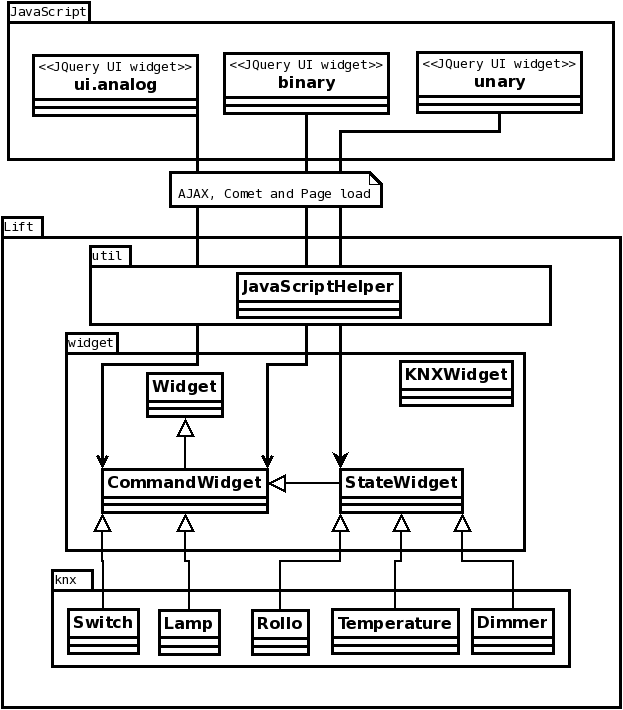
\includegraphics[width=0.80\linewidth]{widgets.png}
  %\input{widgets}
  \caption{widget structure}
  \label{fig:widgets}
  \end{figure}
